\documentclass{article}
\usepackage{graphicx}
\usepackage{geometry}
\usepackage{amsmath}
\usepackage{amsfonts}
\usepackage{tikz}
\usepackage{float}

\geometry{margin=1in}

\title{2024-2025-Autumn-DisMa-8}
\author{2022012050\quad He Yuhui}
\date{November 2024}

\begin{document}

\maketitle

\section{Homework}

\subsection{List the element}

$$
    \begin{aligned}
        A=\{&\{0,-2\},\{0,-1\},\{0,0\},\{0,1\},\\
          &\{1,-2\},\{1,-1\},\{1,0\},\{1,1\},\\
          &\{2,-2\},\{2,-1\},\{2,0\},\{2,1\}\}
    \end{aligned}
$$

\subsection{Write the statememt of the set}

$$
    A=\left\{p\mid\forall q\in\mathbb{N},2\leq q\leq p-1,p\mod q\neq 0\right\}
$$

\subsection{Raise examples}

\quad

Example for 1:

$$
    A=\emptyset,B=\{\emptyset\},C=\{\{\emptyset\}\}
$$

Example for 2:

$$
    A=\emptyset,B=\{\emptyset\},C=\{\emptyset,\{\emptyset\}\}
$$

\subsection{Prove}

\quad

Proof to 1: According to the definition of subset, we know for all elements $x$ in the subset $B$ of set $C$:

$$
    (x\in B)\land (B\subseteq C)\Rightarrow x\in C
$$

and it is similar to the situation that element $x$ is also a set.

\quad

2 is not correct. Consider

$$
    A=\{1, \{2\}\},B=\{\{1, \{2\}\}, 3\},C=\{\{1, \{2\}\}, 3, \{4\}\}
$$

It satisfies $A\in B, B\subseteq C$, but obviously $A\subseteq C$ is false.

\subsection{Write the result}

\quad

The power set of 1:

$$
    \{\emptyset,\{a\},\{\{a\}\},\{a,\{a\}\}\}
$$

The power set of 2:

$$
    \{\emptyset,\{a\},\{\{b\}\}, \{\emptyset,a\},\{\emptyset,\{b\}\},\{a,\{b\}\},\{\emptyset,a,\{b\}\}\}
$$

The power set of 3: we know that $2^{\emptyset}=\{\emptyset\}$, so we have:

$$
    \mathcal{P}(\mathcal{P}(\emptyset))=2^{\{\emptyset\}}=\{\emptyset,\{\emptyset\}\}
$$

so we have 

$$
    \mathcal{P}(\mathcal{P}(\emptyset))\times\mathcal{P}(\mathcal{P}(\emptyset))=\{(\emptyset,\emptyset),(\emptyset,\{\emptyset\}),(\{\emptyset\},\emptyset),(\{\emptyset\},\{\emptyset\})\}
$$

\subsection{Draw the Venn diagram}

$$
    A\cap(-B\cup-C)
$$

\begin{center}
    \begin{minipage}{0.5\textwidth}
        \centering
        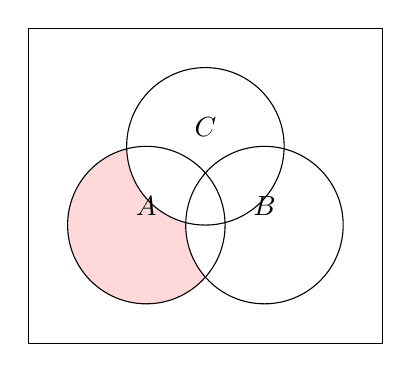
\begin{tikzpicture}
            \begin{scope}
                \clip (0, 0) circle (1);
                \fill[fill=red!50, opacity=0.3] (0, 0) circle (1);
                \fill[fill=white] (0.75, 1) circle (1);
                \fill[fill=white] (1.5, 0) circle (1);
            \end{scope}
            \draw (-1.5, -1.5) rectangle (3, 2.5);
            \draw (0,0) circle (1) node[above] {$A$};
            \draw (1.5, 0) circle (1) node[above] {$B$};
            \draw (0.75, 1) circle (1) node[above] {$C$};
        \end{tikzpicture}
    \end{minipage}
\end{center}

$$
    A\oplus (B\cup C)
$$

\begin{center}
    \begin{minipage}{0.5\textwidth}
        \centering
        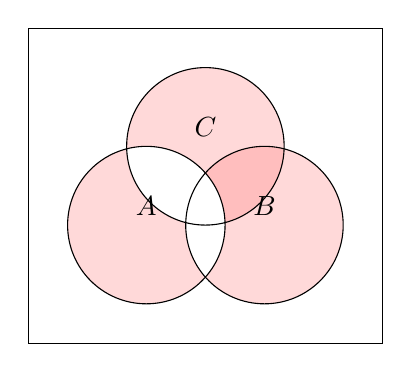
\begin{tikzpicture}
            \begin{scope}
                \clip (0, 0) circle (1);
                \fill[fill=red!50, opacity=0.3] (0, 0) circle (1);
                \fill[fill=white] (0.75, 1) circle (1);
                \fill[fill=white] (1.5, 0) circle (1);
            \end{scope}
            \begin{scope}
                \clip (0.75, 1) circle (1);
                \fill[fill=red!50, opacity=0.3] (0.75, 1) circle (1);
                \fill[fill=white] (0, 0) circle (1);
            \end{scope}
            \begin{scope}
                \clip (1.5, 0) circle (1);
                \fill[fill=red!50, opacity=0.3] (1.5, 0) circle (1);
                \fill[fill=white] (0, 0) circle (1);
            \end{scope}
            \draw (-1.5, -1.5) rectangle (3, 2.5);
            \draw (0,0) circle (1) node[above] {$A$};
            \draw (1.5, 0) circle (1) node[above] {$B$};
            \draw (0.75, 1) circle (1) node[above] {$C$};
        \end{tikzpicture}
    \end{minipage}
\end{center}

\subsection{Write the set}

\quad

The set of Venn diagram 1 is:

$$
    -A\cap B\cap C
$$

The set of Venn diagram 2 is

$$
    -(A\cup B\cup C)\cup(A\cap B\cap C)
$$

\subsection{Write the set}

$$
    -(A\cap B)=\{2,3,4,5\}
$$

$$
    \begin{aligned}
        \mathcal{P}(A)-\mathcal{P}(B)&=\{\emptyset,\{1\},\{4\},\{1,4\}\}-\{\emptyset,\{1\},\{2\},\{5\},\{1,2\},\{1,5\},\{2,5\},\{1,2,5\}\}\\
        &=\{\{4\},\{1,4\}\}
    \end{aligned}
$$

\end{document}
